% %%%%%%%%%%%%%%%%%%%%%%%%%%%%%%%%%%%%%%%%%%%%%%%%%%%%%%%%%%%%%%%%%%%%%%%%%%%%%
\chapter{Non-autoregressive NMT with Connectionist Temporal Classification}
\label{chap:nar-nmt-ctc}
% %%%%%%%%%%%%%%%%%%%%%%%%%%%%%%%%%%%%%%%%%%%%%%%%%%%%%%%%%%%%%%%%%%%%%%%%%%%%%

In this chapter, we lay grounds for the \ac{nar} approaches studied in this
thesis. We describe our experiments with an architecture based on the \ac{ctc}
loss \citep{libovicky-helcl-2018-end}. \JH{ok to self-cite when sections will
  be based on this?} \JH{use \ac{nat} here somewhere}

% -----------------------------------------------------------------------------
\section{Connectionist Temporal Classification}
\label{sec:ctc}
% -----------------------------------------------------------------------------

\Ac{ctc} \citep{graves2006connectionist} is a method for training neural
networks on sequential data. Originally applied to the phonetic labelling task,
but later successfully adapted in related areas, including \ac{asr} or
handwriting recognition \citep{liwicki2007novel, eyben2009speech,
  graves2014towards}.

The main strength of \ac{ctc} becomes evident in tasks where the input and
output labels are weakly or not at all aligned, for example in situations where
the observed input sequence is considerably longer than the target output
sequence -- hence the application to \ac{asr}, where the number of extracted
features per second is higher than the number of phonemes uttered per second.
\JH{Confirm this.}

Training neural networks with \ac{ctc} is independent on the actual neural
network architecture. The \ac{ctc} loss function can be applied on any network
with sequential outputs. Thus, this method is applicable to both \acp{rnn} and
the Transformer model.

Models trained with the \ac{ctc} assume that the alignment between the input
(e.g. a group of frames in an audio signal) and the output (e.g. a phoneme)
states is unknown. A variable number of frames in a row can encode a single
phoneme. Similarly, in translation, multiple words in the source language may
correspond to any number of (even non-consecutive) words in the target
language.

The idea behind \ac{ctc} is to allow some states to produce no output. This is
realized by introducing a special blank token in the target vocabulary.
Optionally, identical outputs produced by multiple consecutive states may be
merged and considered a single output. Because of these properties, there are
groups of equivalent output sequences, which all represent the same target, as
illustrated in Figure~\ref{fig:ctc-equivalent-sequences}.

\begin{figure}
  \centering
  \begin{minipage}{\textwidth}
    \begin{equation*}
        \text{a cat sat on a mat} =
        \begin{cases}
          & \text{a <blank> cat sat on a <blank> mat} \\
          & \text{a a cat cat sat on a mat} \\
          & \text{a <blank> cat cat sat on a mat} \\
        \end{cases}
    \end{equation*}
  \end{minipage}
  \caption{A group of output sequences of equal length which all represent the
    same target in CTC.} %
  \label{fig:ctc-equivalent-sequences}
\end{figure}

In the standard sequence-to-sequence architectures, the value of the loss
function is defined as the sum of the cross entropies of each output state with
respect to the target sequence (see Equation \ref{eq:loss}). In \ac{ctc}, the
loss is defined as the sum of cross-entropy losses of all of the output
sequences equivalent to the given target sequence:
%
\begin{equation}
  J_{\theta}^{\text{CTC}} = - \sum_{(x, y) \in D} \sum_{y' \sim y}  \log p(y' | x, \theta)
  \label{eq:ctc-loss}
\end{equation}
%
where $\sim$ denotes the equivalence relation.  \JH{$J_{\theta}$ should perhaps
  be $J(\theta)$. Also, consider the $\sim$ sign.}

The inner summation in Equation \ref{eq:ctc-loss} is computed over all possible
sequences equivalent to the label sequence. For technical purposes, the label
sequences are limited to a fixed length, which greatly reduces the number of
acceptable hypotheses. However, the number of equivalent hypotheses of a given
length still grows exponentially with the sequence length -- in \ac{ctc}, the
fixed length is always set to be longer than the label sequence. \JH{confirm
  the exponential claim}

The summation over the large set of equivalent sequences can be
implemented using dynamic programming. When both the length of the output and
the length of the target sequences are known, there is a constant number of the
blank tokens to be generated. The process of computing the loss of the whole
output sequence is divided into computing the partial losses with respect to
the possible label prefixes.

\begin{figure}
  \centering

  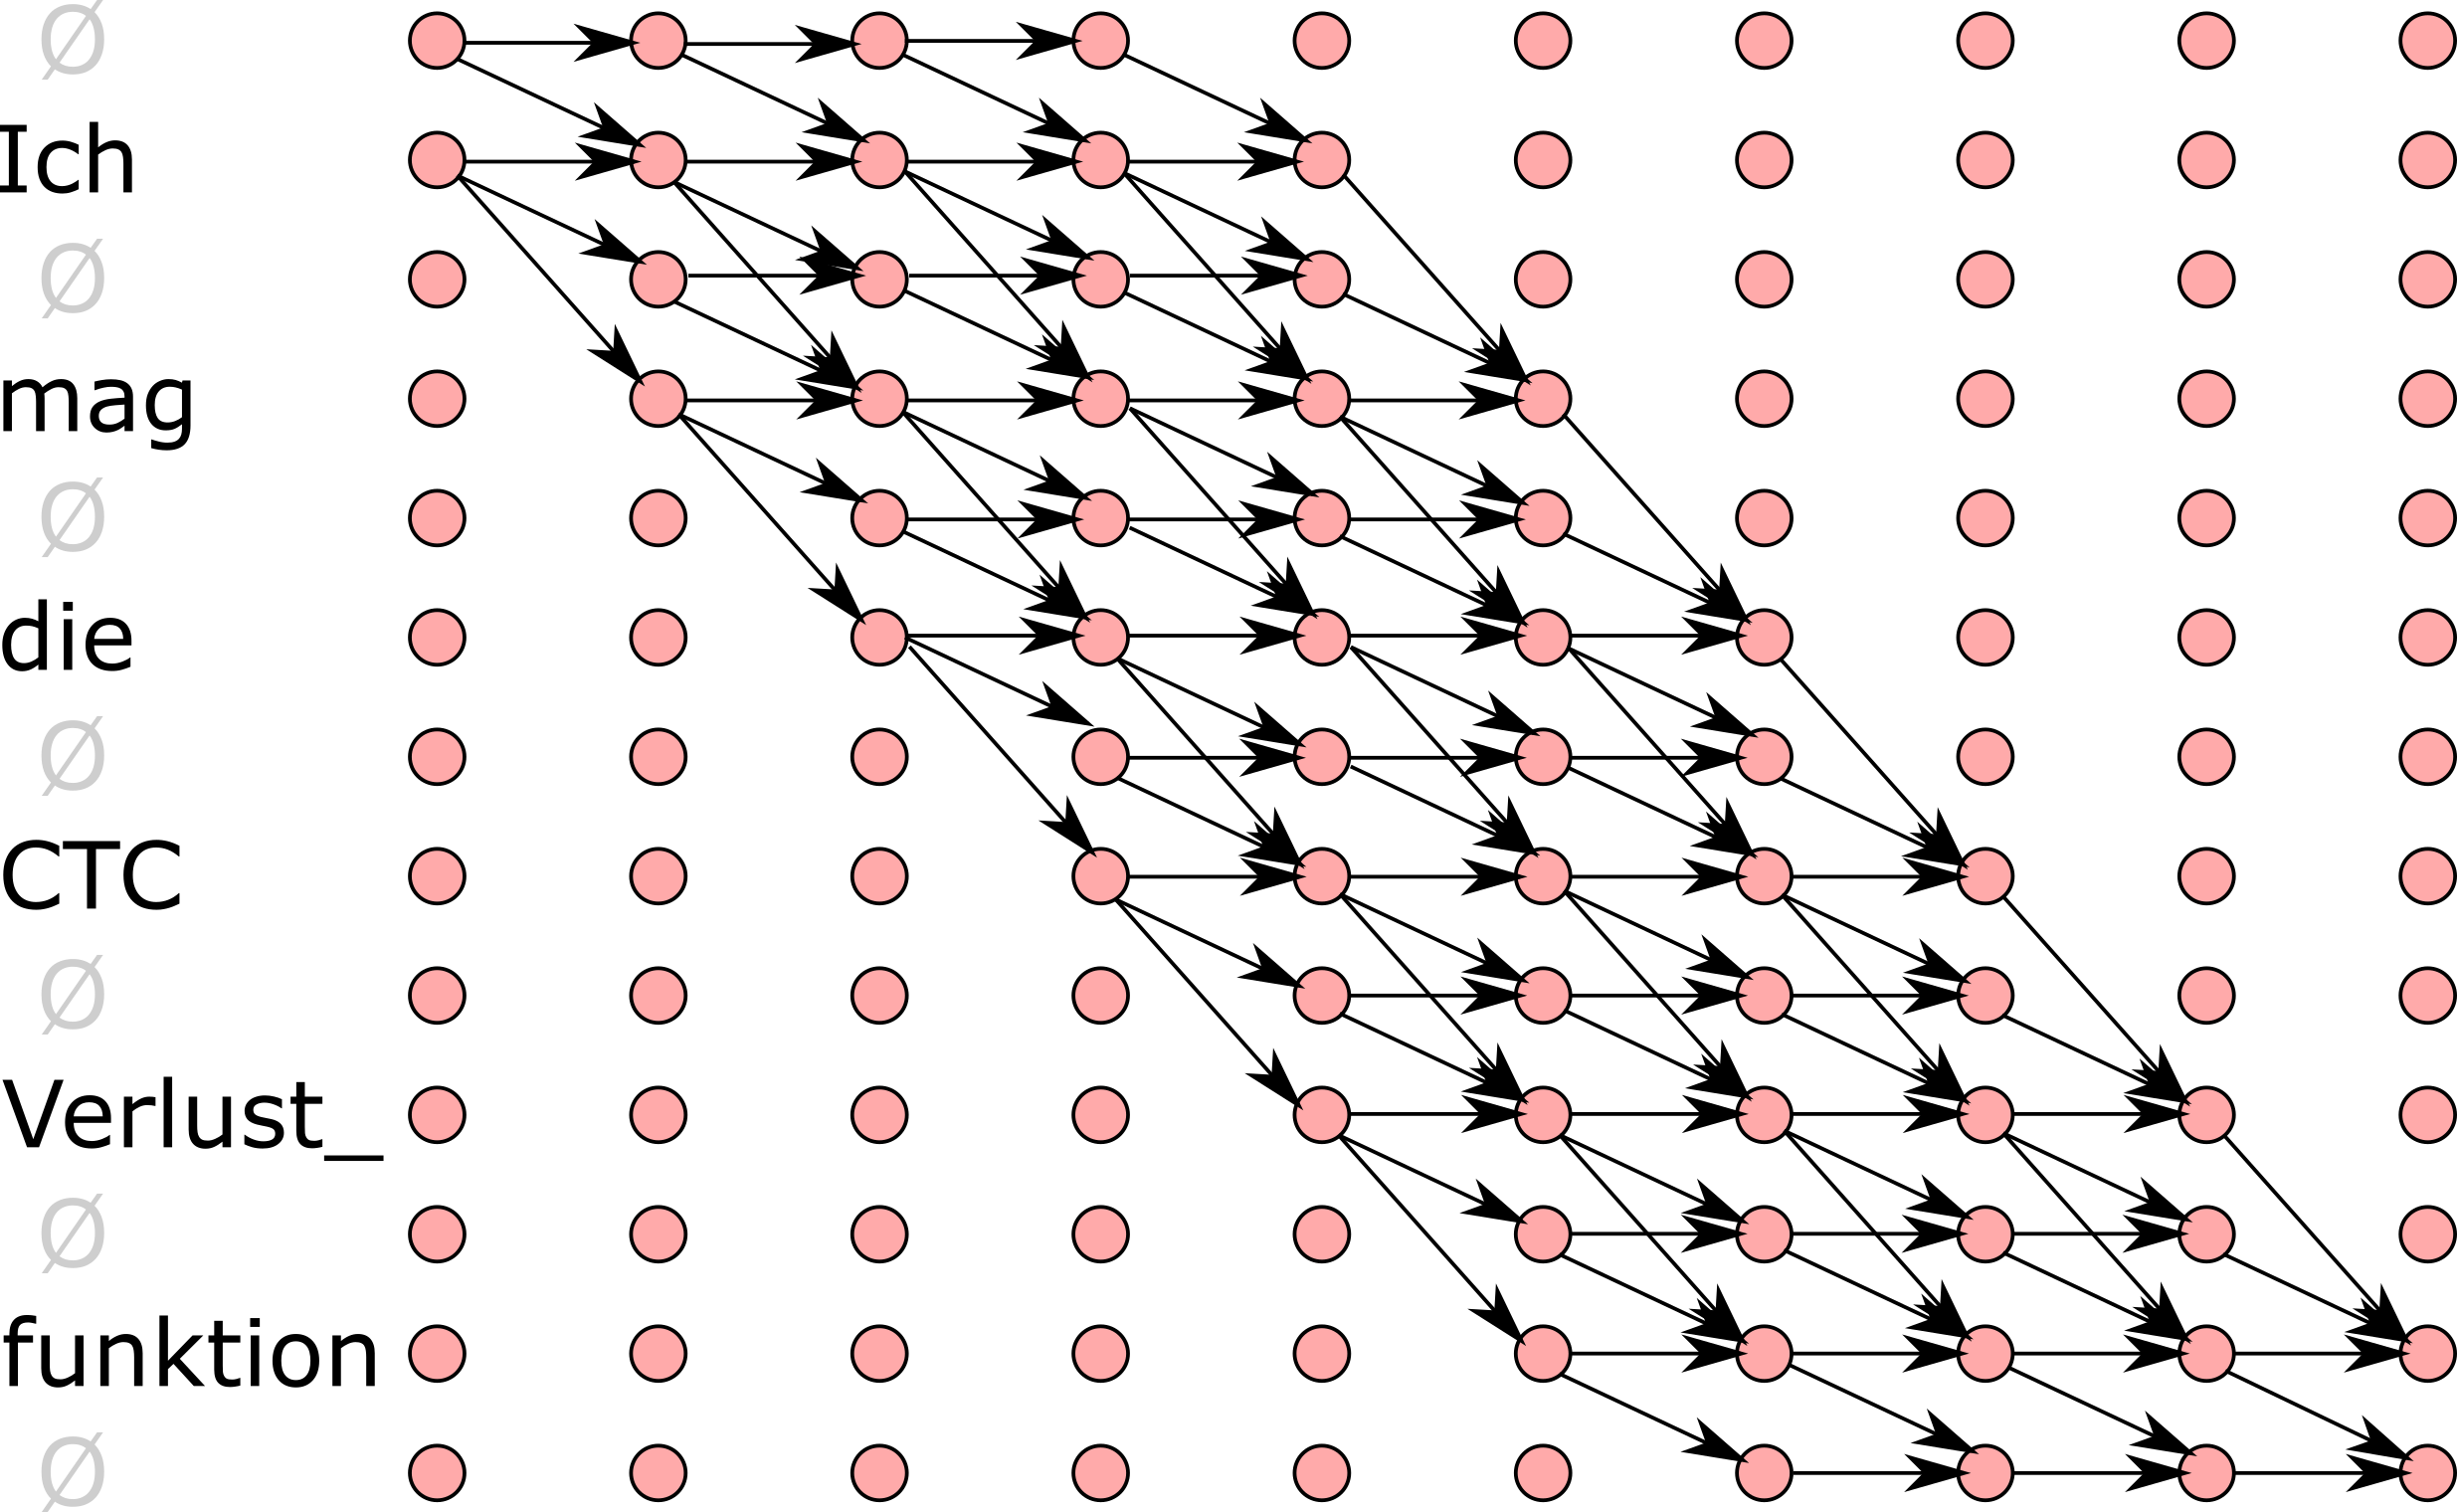
\includegraphics[width=13cm]{img/ctc_schema.png}

  \caption{An illustration of the algorihm for the CTC loss computation. Each
    node denotes producing either a token from the label sequence, or the blank
    token. Each path from one of the two top-left nodes to one of the two
    bottom-right nodes corresponds to one of the equivalent sequences.  }
  \label{fig:ctc-dynamic-programming}
\end{figure}

The \ac{ctc} loss computation is illustrated in Figure
\ref{fig:ctc-dynamic-programming}. The rows represent tokens from the label
sequence plus the optional blank tokens. The columns represent the output state
sequence.  Each node in the graph denotes generating a label from an output
state. The arrows show valid transitions between the generation steps. An arrow
can only go down one or two rows, or horizontally.  The horizontal arrows
denote repeated generation of the same label. These labels are later merged to
form a single output. An arrow can only go two rows down when the skipped row
corresponds to the blank token, so no target tokens are left out. Each path in
the diagram therefore shows one of the equivalent sequences that lead to
generating the given label sequence.

Using the idea that many of the paths from left to right in the diagram share
segments, we can apply dynamic programming to compute the sum of losses across
all paths without the need to enumerate each of them. A node on coordinates
$(i,j)$ stores the accumulated losses for the all path prefixes that lead to
the node, added with the negative log likelihood of the label on the $i$-th row
being generated by the $j$-th output state. The two bottom-right nodes then
store the sum of losses of all the paths.


\JH{doplnit} The training of the network with \ac{ctc} is done by minimizing
the \ac{ctc} loss function, which is defined as follows.

% -----------------------------------------------------------------------------
\section{Model Architecture}
\label{sec:ctc:arch}
% -----------------------------------------------------------------------------

As said in the previous chapter, training models with \ac{ctc} does not impose
any requirements on the model architecture. In our experiments, we aim for a
reasonable comparison between our proposed approach and the state-of-the-art
autoregressive models. We adapt the Transformer model and use similar
hyper-parameters where applicable.

Non-autoregressive models generate the outputs in parallel, which requires that
the output length is known beforehand. In autoregressive models, the end of
sequence is indicated by a special end symbol, and the constraint on maximum
length is merely a technical aspect.

To leverage the ability to output empty tokens to the full extent, the output
length should be set to a higher number than the length of the target sequence.
Since the length estimation does not need to be accurate, we select a number
$k$ and we set the target sequence length to be $k$ times longer than the
source length. Note that in case the selected length is shorter than the label
sequence, the model will not be able to generate the whole target sequence.

\begin{figure}
  \centering
  \def\inputsize{7}

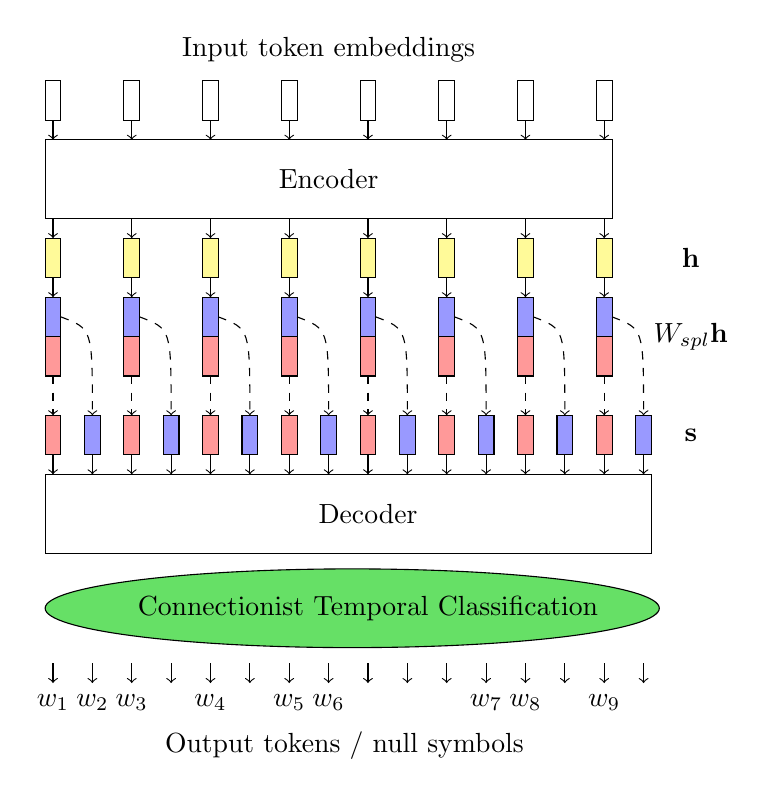
\begin{tikzpicture}[]

\draw (\inputsize / 2 + 0.1, -0.1) node {Input token embeddings};

\foreach \i in {0,...,\inputsize} {
	\draw (\i,-0.5) rectangle (\i+0.2,-1);
    \draw [->] (\i+0.1,-1) -- (\i+0.1, -1.25);
};

\draw (0, -1.25) rectangle (\inputsize + 0.2, -2.25);
\draw (\inputsize / 2 + 0.1, -1.75) node {Encoder};

\foreach \i in {0,...,\inputsize} {
	\draw [->] (\i+0.1,-2.25) -- (\i+0.1, -2.5);
    \draw[fill=yellow!40] (\i,-2.5) rectangle (\i+0.2,-3);

    \draw [->] (\i+0.1,-3) -- (\i+0.1, -3.25);
	\draw[fill=blue!40] (\i,-3.25) rectangle (\i+0.2,-3.75);
	\draw[fill=red!40] (\i,-3.75) rectangle (\i+0.2,-4.25);

    \draw [dashed,->] (\i+0.1,-4.25) -  - (\i+0.1, -4.75);
    \draw [dashed,->] (\i+0.2,-3.5) .. controls (\i + 0.6, -3.65) .. (\i+0.6, -4.75);

	\draw[fill=red!40] (\i,-4.75) rectangle (\i+0.2,-5.25);
	\draw[fill=blue!40] (\i + 0.5,-4.75) rectangle (\i+0.7,-5.25);

    \draw [->] (\i+0.1,-5.25) - - (\i+0.1, -5.5);
    \draw [->] (\i+0.6,-5.25) - - (\i+0.6, -5.5);
};

\draw (\inputsize + 1.2, -2.75) node {$\mathbf{h}$};
\draw (\inputsize + 1.2, -3.75) node {$W_{\text{spl}}\mathbf{h}$};
\draw (\inputsize + 1.2, -5.00) node {$\mathbf{s}$};

\draw (0, -5.5) rectangle (\inputsize + 0.7, -6.5);
\draw (\inputsize / 2 + 0.5 + 0.1, -6.0) node {Decoder};

\draw [fill=green!80!black!60] (\inputsize / 2 + 0.4,-7.2) circle [x radius=\inputsize / 2 + 0.4, y radius=0.5];
\draw (\inputsize / 2 + 0.6, -7.2) node {Connectionist Temporal Classification};

\foreach \i in {0,...,\inputsize} {
   \draw [->] (\i+0.1,-7.9) - - (\i+0.1, -8.15);
   \draw [->] (\i+0.6,-7.9) - - (\i+0.6, -8.15);
}

\draw  (0+0.1,-8.4) node {$w_1$};
\draw  (0+0.6,-8.4) node {$w_2$};
\draw  (1+0.1,-8.4) node {$w_3$};
\draw  (1+0.6,-8.4) node {$\varnothing$};
\draw  (2+0.1,-8.4) node {$w_4$};
\draw  (2+0.6,-8.4) node {$\varnothing$};
\draw  (3+0.1,-8.4) node {$w_5$};
\draw  (3+0.6,-8.4) node {$w_6$};
\draw  (4+0.1,-8.4) node {$\varnothing$};
\draw  (4+0.6,-8.4) node {$\varnothing$};
\draw  (5+0.1,-8.4) node {$\varnothing$};
\draw  (5+0.6,-8.4) node {$w_7$};
\draw  (6+0.1,-8.4) node {$w_8$};
\draw  (6+0.6,-8.4) node {$\varnothing$};
\draw  (7+0.1,-8.4) node {$w_9$};
\draw  (7+0.6,-8.4) node {$\varnothing$};

\draw (\inputsize / 2 + 0.3, -8.95) node {Output tokens / null symbols};

\end{tikzpicture}

  \caption{The scheme of the non-autoregressive architecture with
    state-splitting and CTC. The image is taken from
    \citet{libovicky-helcl-2018-end}.}%
  \label{fig:state-splitting}
\end{figure}


We implement the source-to-target length expansion by linear projections and
state splitting. This mechanism is illustrated in Figure
\ref{fig:state-splitting}. After a given Transformer layer completes its
computation, we linearly project the states
$h_1, \ldots, h_{T_x} \in \mathbb{R}^d$ into $\mathbb{R}^{kd}$. Then, we split
each of these projections into $k$ parts, which results to a $k$-times longer
sequence of states $s_1, \ldots, s_{k \cdot T_x}$ of the original dimension
$d$:
%
\begin{equation}
  s_{ck+b} = \left( W_{\text{spl}} h_c + b_{\text{spl}} \right)_{bd:(b+1)d}
\end{equation}
%
for $b=0 \ldots k-1$ and $c=1 \ldots T_x$ where
$W_{\text{spl}} \in \mathbb{R}^{d \times kd}$ and
$b_{\text{spl}} \in \mathbb{R}^{kd}$ are the trainable projection parameters.

We experiment with two placement options of the state splitting layer. First,
we try placing the state splitting at the end of the Transformer layer
stack. In this scenario, there are 12 Transformer encoder layers, followed by
the state splitting layer, whose outputs are used in the output
projection. Second, we place the state splitting layer in the middle of the
Transformer layer stack, mimicking the 6-layer encoder-decoder architecture of
the autoregressive Transformer model. In the second variant, cross-attention
can be included in the second half of the layers, which attends to the states
right after state splitting.

% -----------------------------------------------------------------------------
\section{Preliminary Experiments}
\label{sec:ctc:experiments}
% -----------------------------------------------------------------------------

\JH{Section with experiments from the 2018 paper. Should show that it works,
  but it's still far from perfect.}

We conduct experiments with \ac{ctc}-based \ac{nat} models trained on
English--German and English--Romanian translation in both directions.

\paragraph{Data.}
In our experiments, we use the parallel data provided by the \acs{wmt}
organizers. For English--German, the training data consist of the Europarl
corpus \citep{koehn-2005-europarl}, News commentary
\citep{tiedemann-2012-parallel}, and Common
Crawl.\footnote{\url{https://commoncrawl.org/}} For validation, we use the
WMT~13 test set \citep{bojar-etal-2013-findings}, and we evaluate the
translation quality on the WMT~14 test set
\citep{bojar-etal-2014-findings}. For English--Romanian, the data consist of
the Europarl corpus, and the SETIMES corpus distributed by OPUS
\citep{tiedemann-2012-parallel}. We use the development and test set from
WMT~16 \citep{bojar-etal-2016-findings}. The data sizes are shown in
Table~\ref{tab:end-to-end:data}.

\begin{table}
  \centering
  \begin{tabular}{lr}
    \toprule
     & Sentence pairs \\
    \midrule
    En -- De & 4.58 M \\
    En -- Ro & 613 k \\
    \bottomrule
  \end{tabular}

  \caption{The training data sizes. \JH{more}}%
  \label{tab:end-to-end:data}
\end{table}

We preprocess the data with scripts from the \texttt{mosesdecoder}
repository,\footnote{\url{https://github.com/moses-smt/mosesdecoder/}} a part
of the Moses translation toolkit \citep{koehn-etal-2007-moses}. Namely, we
normalize the punctuation in the data, then we use the tokenizer and a
truecaser. We segment the data using the wordpiece algorithm, creating a
vocabulary of 32,000 tokens \citep{wu2016google}.

\paragraph{Models and Training.}
We implement and train our models in the Neural Monkey toolkit
\citep{helcl-libovicky-2017-neural,helcl-etal-2018-neural}. Neural Monkey is a
higher-level deep learning toolkit implemented in TensorFlow
\citep{tensorflow2015-whitepaper}, aiming for fast prototyping using
simple-format configuration files. We train all models for 10 epochs and we
select the best-scoring model based on the validation BLEU score. The training
of the En--De models on a single Nvidia GeForce GTX 1080 GPU took approximately
4 weeks. Since the En--Ro parallel data was much smaller, the training of the
En--Ro models took 4 days.

We summarize the model and training settings in Table
\ref{tab:end-to-end:hparams}. Note that the architecture resembles the
Transformer big settigns, but uses a smaller model dimension. We use the same
settings for training models in both directions in both language pairs.

\begin{table}
  \centering
  \begin{tabular}{lr}
    \toprule
    Parameter & Value \\
    \midrule
    No. of encoder layers & 6 \\
    No. of decoder layers & 6 \\
    Model dimension & 512 \\
    Attention heads & 16 \\
    Dropout probability & 0.1 \\
    Feed-forward hidden size & 4096 \\
    State splitting factor & 3 \\
    State splitting projection size & 1536 \\
    Vocabulary size & 32,000 \\
    \midrule
    Optimizer method & adam \\
    $\beta_1$ & 0.9 \\
    $\beta_2$ & 0.997 \\
    $\epsilon$ & 10$^{-9}$ \\
    Learning rate & 10$^{-4}$ \\
    Fixed batch size & 20 \\
    Gradient clip norm & 1 \\
    \bottomrule
  \end{tabular}

  \caption{Experimental settings for the Neural Monkey experiments.}%
  \label{tab:end-to-end:hparams}
\end{table}

\paragraph{Results.} Table \ref{tab:end-to-end:bleu} compares the quantitative
results of our non-autoregressive models with methods proposed by
\citet{gu2017nonautoregressive} and \citet{lee-etal-2018-deterministic}. We use
the SacreBLEU \citep{post-2018-call} to compute the BLEU scores of the model
outputs.

\begin{table}
  \centering
  \begin{tabular}{lcccc}
    \toprule
     & \multicolumn{2}{c}{WMT~16} & \multicolumn{2}{c}{WMT~14} \\
     & En $\rightarrow$ Ro & Ro $\rightarrow$ En & En $\rightarrow$ De & De $\rightarrow$ En \\
    \midrule
    \citet{gu2017nonautoregressive} & & & & \\
    Autoregressive baseline & 31.35 & 31.03 & 22.71 & 26.39 \\
    NAT + FT & 27.29 & 29.06 & 17.69 & 21.47 \\
    NAT + FT + NPD (100 s) & 29.79 & 31.44 & 19.17 & 23.20 \\
    \midrule
    \citet{lee-etal-2018-deterministic} & & & & \\
    Autoregressive baseline & 31.93 & 31.55  & 23.77 & 28.15 \\
    1 iteration & 24.45 & 25.73 & 13.91 & 16.77 \\
    10 iterations & 29.32 & 30.19 & 21.61 & 25.48 \\
    \midrule
    \citet{libovicky-helcl-2018-end} & & & & \\
    Autoregressive baseline & 21.19 & 29.64 & 22.94 & 28.58 \\
    Deep encoder & 17.33 & 22.85 & 12.21 & 12.53 \\
    + weight averaging & & & & \\
    + beam search & & & & \\
    Encoder-decoder  & & & & \\
    + weight averaging & 19.54 & 24.67 & 16.56 & 18.64 \\
    + beam search & & & & \\
    Encoder-decoder with pos. encoding  & & & & \\
    + weight averaging & & & & \\
    + beam search & 19.93 & 24.71 & 17.68 & 19.80 \\
    \bottomrule
  \end{tabular}

  \caption{Automatic evaluation of our \acs{ctc}-based approach, compared to
    the two of the first non-autoregressive methods.}%
  \label{tab:end-to-end:bleu}
\end{table}




\paragraph{Limitations.} \JH{List all the limitations here: namely, no
  knowledge distillation}

%%% Local Variables:
%%% mode: latex
%%% TeX-master: "thesis"
%%% End:
